\documentclass[11pt]{article}
\usepackage[utf8]{inputenc}
\usepackage{geometry}
\usepackage{url}
\usepackage{hyperref}
\usepackage{epsfig}
\usepackage{graphicx}
\usepackage[most]{tcolorbox}
\geometry{a4paper}
\geometry{margin=0.75in}

\usepackage[sorting=none, backend=bibtex]{biblatex}
\usepackage{filecontents}
\usepackage{tabularx}

\def\etal{\emph{et al}.\ }
\newcommand{\CPP}
{C\nolinebreak[4]\hspace{-.05em}\raisebox{.22ex}{\footnotesize\bf ++\ }}

\begin{filecontents}{intermediate-report-references.bib}

@inproceedings{le2014distributed,
  title={Distributed Representations of Sentences and Documents.},
  author={Le, Quoc V and Mikolov, Tomas},
  booktitle={ICML},
  volume={14},
  pages={1188--1196},
  year={2014}
}

@misc{wikidatadump2016,
  author="Meta",
  title="Data dump torrents --- Meta{,} discussion about Wikimedia projects",
  year="2016",
  url={https://meta.wikimedia.org/w/index.php?title=Data_dump_torrents},
  note="[Online; accessed 9-August-2016]"
}

@inproceedings{broder1997resemblance,
  title={On the resemblance and containment of documents},
  author={Broder, Andrei Z},
  booktitle={Compression and Complexity of Sequences 1997. Proceedings},
  pages={21--29},
  year={1997},
  organization={IEEE}
}

@misc{keras,
  title={Keras: Deep Learning library for Theano and TensorFlow},
  url={https://keras.io/}
}

@inproceedings{gensim,
  title = {{Software Framework for Topic Modelling with Large Corpora}},
  author = {Radim {\v R}eh{\r u}{\v r}ek and Petr Sojka},
  booktitle = {{Proceedings of the LREC 2010 Workshop on New
       Challenges for NLP Frameworks}},
  pages = {45--50},
  year = 2010,
  month = May,
  day = 22,
  publisher = {ELRA},
  address = {Valletta, Malta},
  note={\url{http://is.muni.cz/publication/884893/en}},
  language={English}
}

@misc{chromium2016,
  title={Git repositories on chromium},
  url={https://chromium.googlesource.com/},
  journal={chromium Git repositories}
}

@InProceedings{maas2011,
  author    = {Maas, Andrew L.  and  Daly, Raymond E.  and  Pham, Peter T.  and  Huang, Dan  and  Ng, Andrew Y.  and  Potts, Christopher},
  title     = {Learning Word Vectors for Sentiment Analysis},
  booktitle = {Proceedings of the 49th Annual Meeting of the Association for Computational Linguistics: Human Language Technologies},
  month     = {June},
  year      = {2011},
  address   = {Portland, Oregon, USA},
  publisher = {Association for Computational Linguistics},
  pages     = {142--150},
  url       = {http://www.aclweb.org/anthology/P11-1015}
}

@article{maaten2008visualizing,
  title={Visualizing data using t-SNE},
  author={Maaten, Laurens van der and Hinton, Geoffrey},
  journal={Journal of Machine Learning Research},
  volume={9},
  number={Nov},
  pages={2579--2605},
  year={2008}
}

\end{filecontents}
\addbibresource{intermediate-report-references.bib}


\title {
  \Huge Mining Big Data - Intermediate Report\\
  \vspace{1em}
  \huge Investigating Paragraph Vectors
}

\author {
  \begin{tabular}{r l}
  a1632538 & Zachary Forman\\
  a1646930 & James Caddy\\
  \end{tabular}
}

\begin{document}

% Cover Page
\pagenumbering{gobble}
\maketitle
\newpage

\section*{Introduction}
  This document describes our progress towards achieving our project goals.
  We have three primary project goals:
  \begin{enumerate}
    \item Replicate the results claimed by Le and Mikolov in their $2014$
          paper~\cite{le2014distributed}.
    \item Compare \texttt{\texttt{doc2vec}} backed with k-nearest-neighbours with
          standard approaches to determining document similarity
          ~\cite{broder1997resemblance}.
    \item Apply \texttt{\texttt{doc2vec}} to source code, and explore how it distributes
          code segments.
  \end{enumerate}
  Our work so far has mostly been towards the first and second of these goals.

\section*{Current Progress}
  \subsection*{Work on the IMDB dataset}
    Some exploratory analysis and testing, using gensim~\cite{gensim}
    as an implementation of \texttt{doc2vec}, and the tests have been run as per
    the paper~\cite{le2014distributed}. So far the results are disappointing.
    Despite several attempts to replicate the paper's experiment, and obtain
    a working sentiment classifier, so far, we have not come close to achieving
    the accuracy described in the paper, or achieved by other approaches. So far,
    only an accuracy of 68\% has been obtained, in contrast with the 92\% claimed
    by Le and Mikolov.

  \subsection*{Work on the Wikipedia dataset}
    We again used gensim~\cite{gensim} to run \texttt{doc2vec} on the wikipedia
    corpus~\cite{wikidatadump2016}. Even with only 2 training iterations on the
    corpus (compared with a desired 10-20), this took over 100 CPU hours.
    From the word and paragraph vectors trained on this data, we
    qualitatively evaluated the algorithm's performance on three axes:
    \begin{enumerate}
      \item Did the learned word vectors capture semantic meaning well?
      \item Did the learned document vectors capture semantic meaning well?
      \item Could the document vectors be used for similarity analysis?
    \end{enumerate}

\section*{Current Experimental Progress}
  All source code necessary to reproduce our results is available at
  \url{https://github.com/mbd-doc2vec-team/mbd-doc2vec/}, the IMDB dataset is
  available as referenced in Maas \etal's work~\cite{maas2011}, and the wikipedia
  dataset is available at~\cite{wikidatadump2016}.
  \subsection*{Experiments on the IMDB Dataset}
    The approach taken followed the method described in the paper as best as possible.
    Gensim~\cite{gensim} was used for the \texttt{doc2vec} implementation, with parameters as
    in Table~\ref{tab:params} and Keras~\cite{keras} backed with Theano was chosen for
    the neural network library, since neither were specified in the paper. It is unlikely
    that either of these choices were the cause for low performance, and more likely
    that our implementation was flawed. Both of these libraries were relatively easy
    to use which was good.\\
    While the paper gives clear descriptions of most components and parameters in the
    classifier architecture, critical details are overlooked and explained poorly.
    Replicating the results without clear descriptions or values falls to trial and
    error, where any number of confounding variables could be in effect.
    One such ambiguity is the dimension of the document vectors, which can have
    large effects on accuracy.

  \subsection*{Experiments on the Wikipedia Dataset}
    Similarly to the IMDB dataset, we

  \begin{table*}
    \begin{center}
      \begin{tabular}{l l l}
        Parameter & IMBD model & Wikipedia model\\
        \hline
        Vector size & 200 & 200\\
        Context distance & 5 & 8\\
        Training iterations & 20 & 2\\
      \end{tabular}
    \caption{Parameters used for \texttt{doc2vec} for each experiment}
    \label{tab:params}
    \end{center}
  \end{table*}

\section*{Future Work}
  \subsection*{IMDB Dataset}
    Further clarification of the architecture would improve the performance far better
    than continued tuning. Unless there is any insight disclosed in discussion around
    the paper, contacting the author of the paper seems like the only way this might be
    achieved. Which is unfortunate, given the author has been so far unwilling to
    help others in discussion groups.
    In order to obtain higher accuracy, there is the possibility that running the
    training for longer could help. Both the embedding and the classifier could benefit
    from this, however over-fitting the data is a concern.
    Currently, achieving an accuracy within 10\% of that claimed by Le
    and Mikolov~\cite{le2014distributed} seems unlikely, and as such, serves as
    a goal for our next experiments.

  \subsection*{Wikipedia Dataset}
    The most pressing, and most time-consuming, future work for the Wikipedia dataset
    is to train the model for more generations. While the word vectors and document
    vectors were somewhat coherent, there was clearly noise caused by under-fitting.
    While training for 20 generations will take $1000$ CPU hours, the benefits of
    training for a significant number of iterations should be worthwhile.\\
    After this, we will compare the similarity metric that can be obtained using
    \texttt{doc2vec} with those obtained from the k-shingles method, particularly
    with intent to quantitatively compare the speed of finding similar documents, and
    qualitatively assess how well the similarity metric compares to a human notion of
    similarity.

  \subsection*{Chromium Dataset}
    % TODO

\newpage

\printbibliography

\section*{Appendices}

  \begin{table*}[h]
    \begin{center}
      \begin{tabular}{l l}
        Wikipedia model & IMBD model\\
        \hline
        apricot & kahuna\\
        cherry & mines\\
        onion & interpreters\\
        mango & explosive\\
        persimmon & imperialist\\
        indigo & catholic\\
        hazelnut & conservatory\\
        pomegranate & pilling\\
        yahoo & craftsmanship\\
        ibm & casing\\
      \end{tabular}
    \caption{Words similar to `apple'}
    \label{tab:apple}
    \end{center}
  \end{table*}

  \begin{table*}[h]
    \begin{center}
      \begin{tabular}{l l}
        Wikipedia model & IMBD model\\
        \hline
        screwball & screwball\\
        slapstick & slapstick\\
        erotic & romance\\
        modernist & stand-up\\
        realist & slap-stick\\
        satirical & physical\\
        absurdist & teen\\
        bromantic & sophisticated\\
        improvisational & erotic\\
        surreal & frothy\\
      \end{tabular}
    \caption{Words similar to `romantic'}
    \label{tab:romantic}
    \end{center}
  \end{table*}

  \begin{figure}[h]
    \begin{center}
      \tcbox{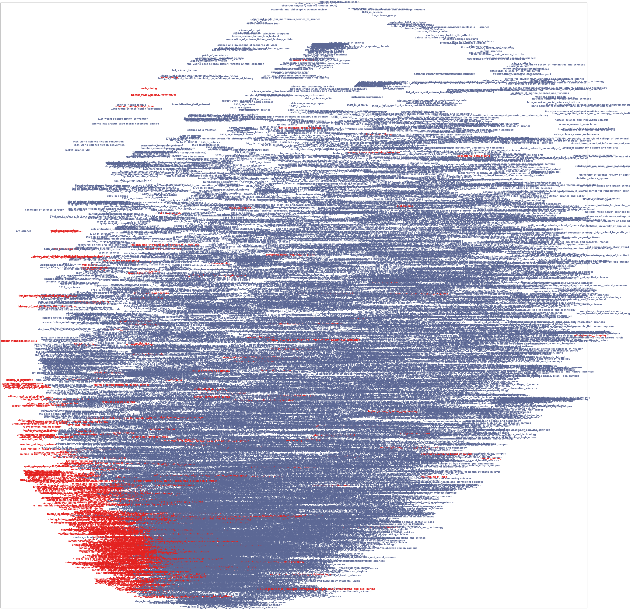
\includegraphics[width=0.7\linewidth]{mining-vs-science.png}}
    \end{center}
    \caption{t-sne~\cite{maaten2008visualizing} used to visualize
             mining (red) and science (blue) wikipedia pages.
             Concepts such as `School of Geological Sciences' are nearer
             the meeting point of the groups.}
    \label{fig:mvs}
  \end{figure}

  \begin{figure}[h]
    \begin{center}
      \tcbox{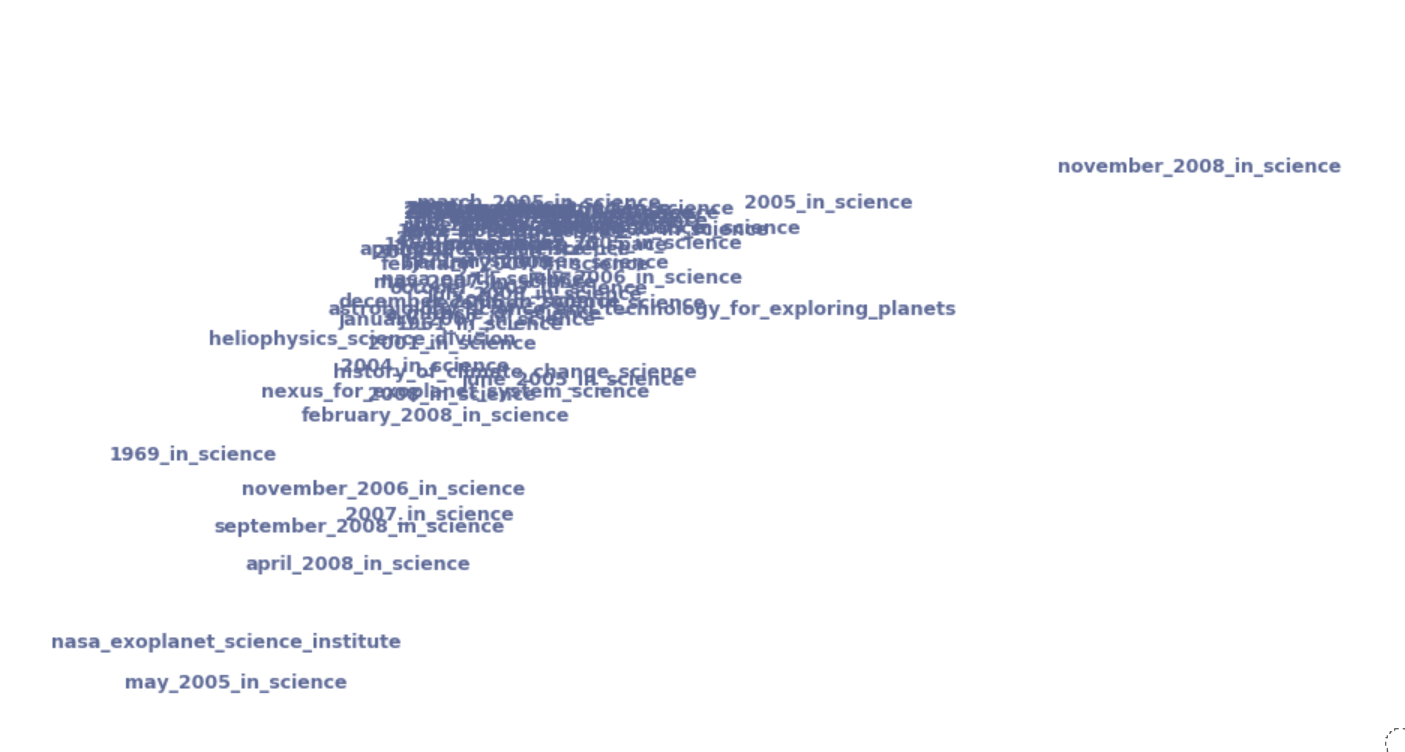
\includegraphics[width=0.7\linewidth]{years_in_science_cluster.png}}
      \tcbox{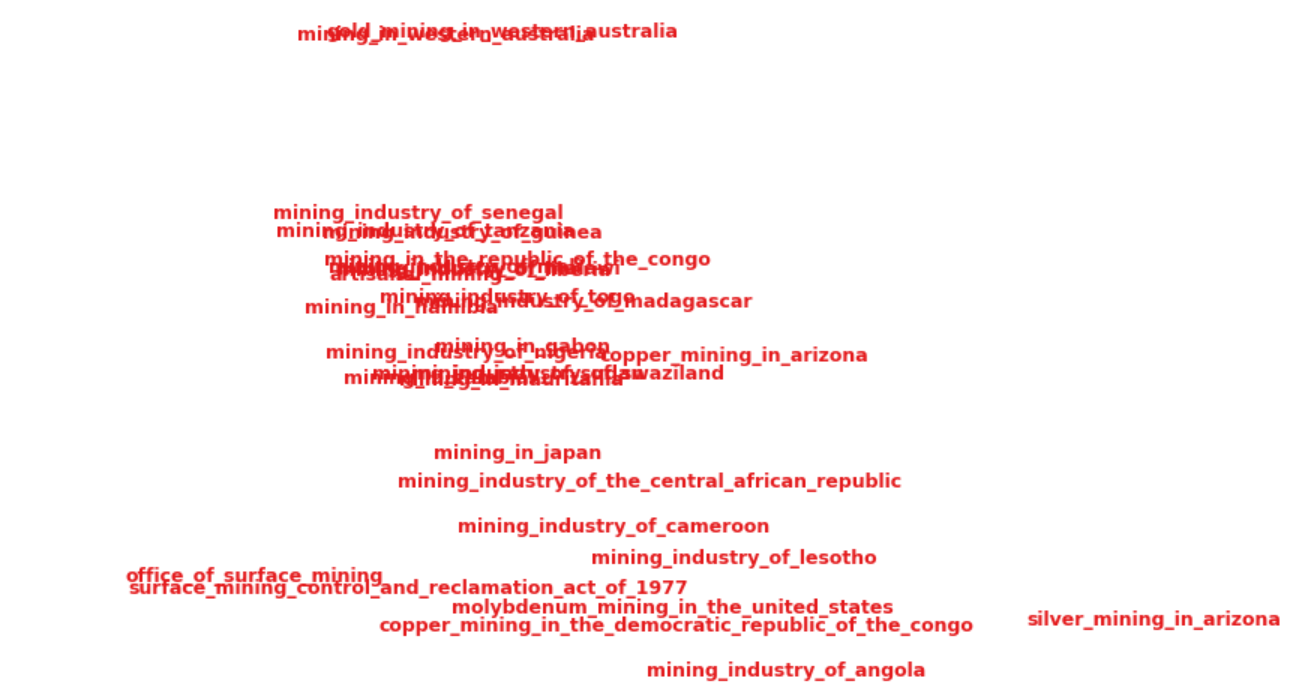
\includegraphics[width=0.7\linewidth]{mining_in_region_cluster.png}}
      \tcbox{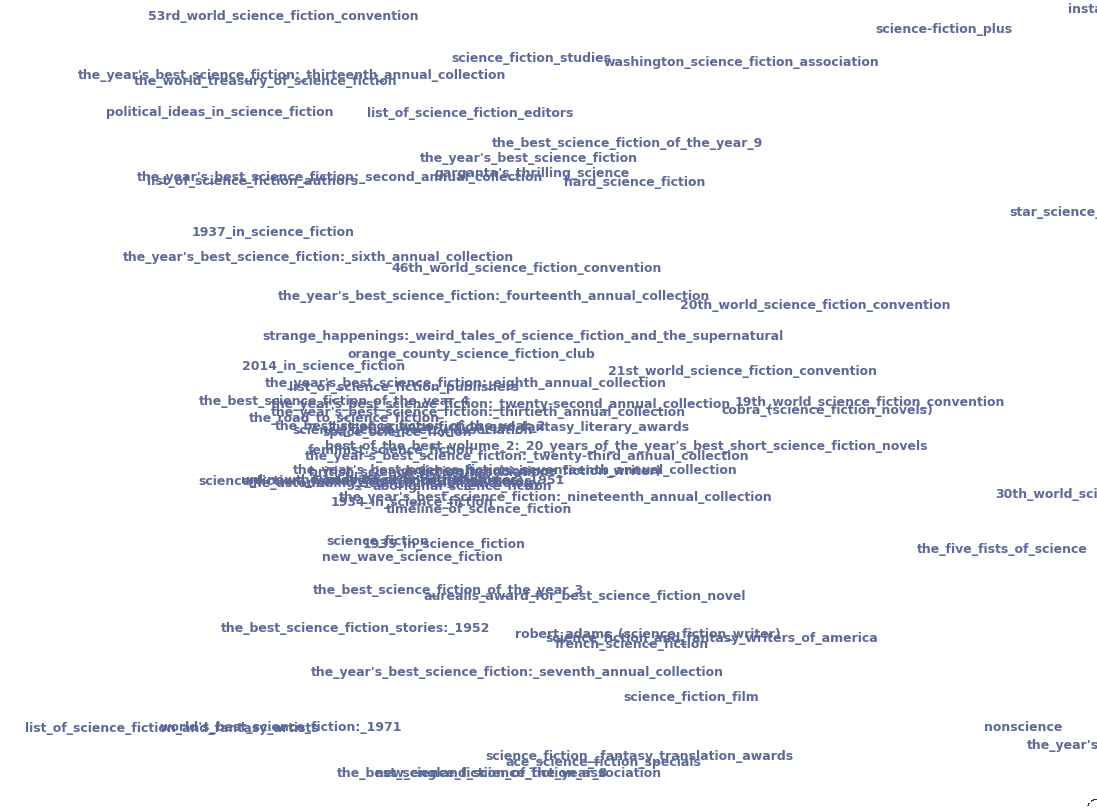
\includegraphics[width=0.7\linewidth]{scifi_cluster.png}}
    \end{center}
    \caption{Some conceptual clusters from Figure~\ref{fig:mvs}.}
    \label{fig:mvssub}
  \end{figure}

  \begin{figure}[h]
    \begin{center}
      \tcbox{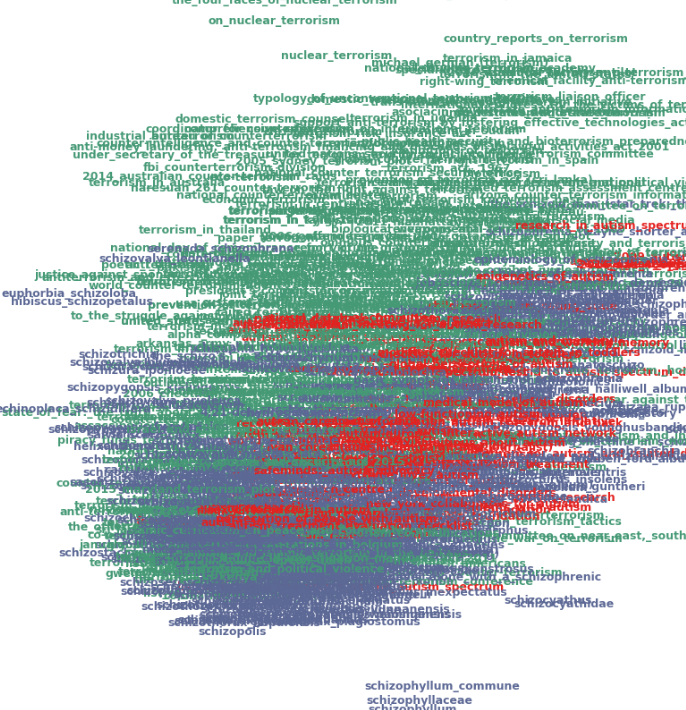
\includegraphics[width=0.7\linewidth]{ast.png}}
    \end{center}
    \caption{t-sne~\cite{maaten2008visualizing} used to visualize
             autism (red), terrorism (blue) and schizo.* (blue)
             Wikipedia pages. Note how autism and schizophrenia are
             clustered together, in the top right.}
    \label{fig:ast}
  \end{figure}

  \begin{figure}[h]
    \begin{center}
      \tcbox{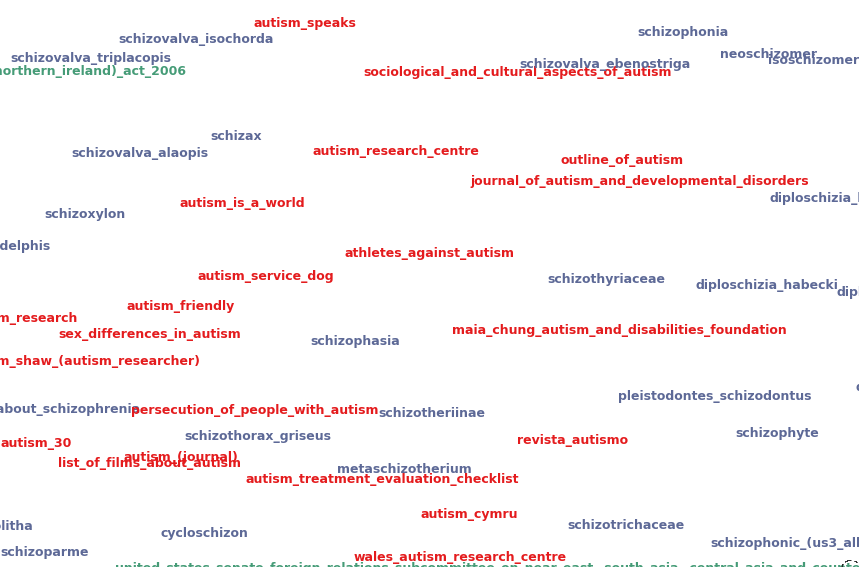
\includegraphics[width=0.7\linewidth]{autism_cluster.png}}
      \tcbox{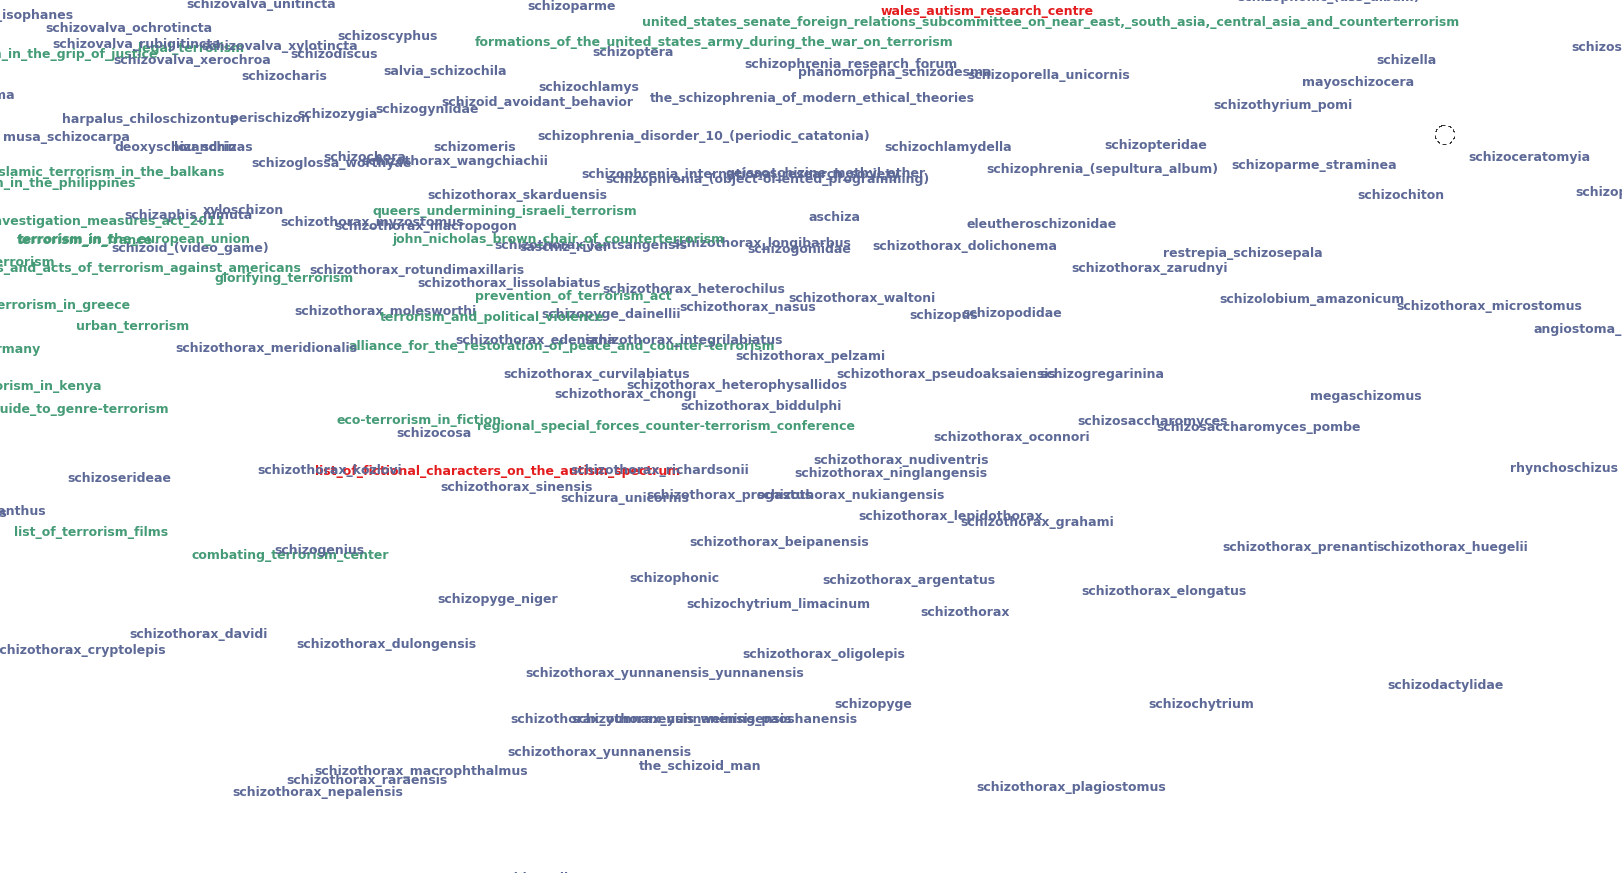
\includegraphics[width=0.7\linewidth]{schizothorax_cluster.png}}
      \tcbox{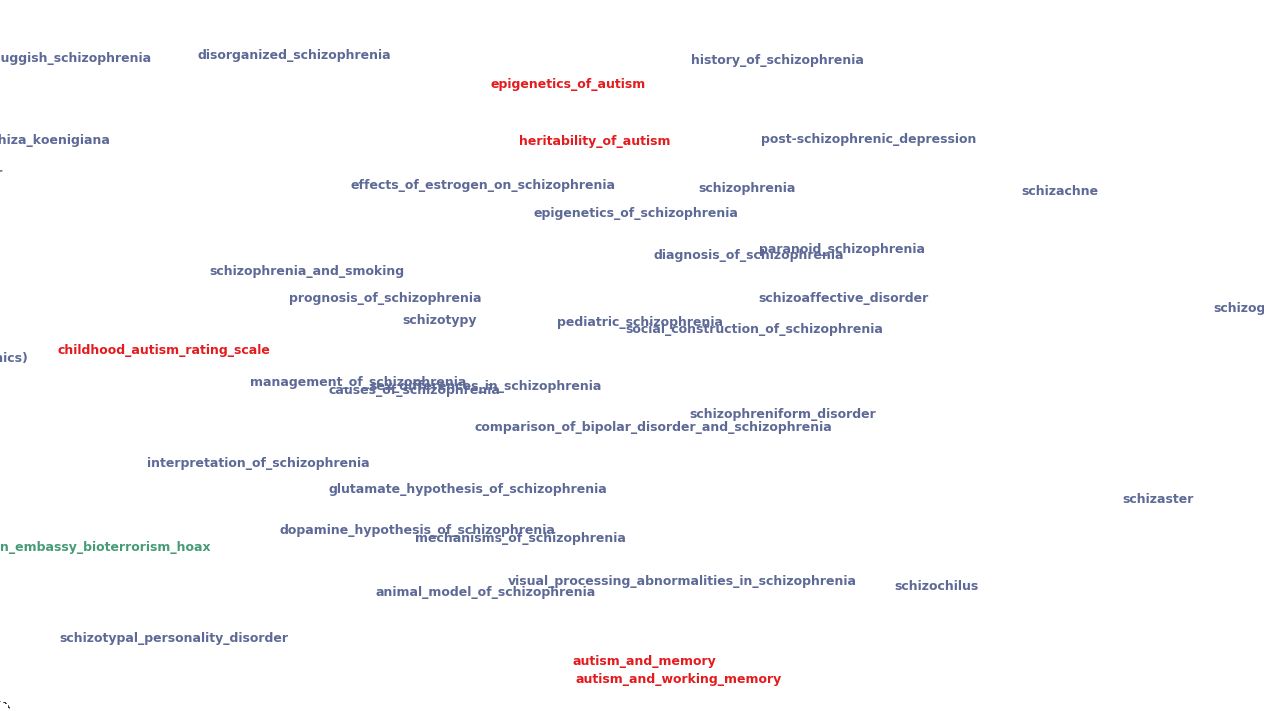
\includegraphics[width=0.7\linewidth]{schizo_cluster.png}}
    \end{center}
    \caption{Some conceptual clusters from Figure~\ref{fig:ast}.}
    \label{fig:mvssub}
  \end{figure}


\end{document}
